\section{Paper Description}

For this project, ``Fast Obstacle Detection Using U-Disparity Maps with Stereo Vision'' was chosen
as it represents a relevant application of the stereo vision principle, as well as adding improvements
to the iterpretation of disparity maps in order to determine scene depth.

The paper present the base techniques used in determining depth from as stereoptic camera system, and
provides a variable thresholding step for determining disparity, as well as two distinct depth map 
enhancement for greater accuracy in obstacle classification.

\subsection{Motivation}

As obstacle detection is a key step towards fully autonomous driving vehicles, the accuracy of determining
the 3-dimensional positions of surrounding objects becomes a necessary hurdle to overcome. For this purpose,
stereovision systems provide ``dense 3D data'', with good accuracy for driving assistance applications. At
the same time, further exploitation of the resulting depth information can lead to more intricate 
applications, such as obstacle classification.~\cite{withMain}

The paper presents an algorithm based on the ``widely used u- and v-disparity concepts'', with the caveat
that the threshold for longer distances does not need to be calibrated a priori, but is instead adapted
dynamically to scene conditions. It also implements a vertical enhancement step, meant to improve obstacle
classification, and a horizontal enhancement step, used to separate the road surface from the rest of the
environment.~\cite{withMain}

\subsection{Implementation}

The detection algorithm begins with the formation of the U-Disparity map, denoted \(U\), recording the amount 
of ``appearances of disparity values in a column wise manner''.  This step involves ``iterating through the
disparity image and incrementing the u-disparity map location'', with the row position in \(U\) representing
the disparity value of the given pixel, and the column position of \(U\) corresponding to the column location 
of the pixel. Likewise, the V-Disparity map, \(V\), is formed in a row wise manner, with the disparity value
being encoded inside each column and the pixel rows being translated.~\cite{withMain}

\begin{figure}[H]
    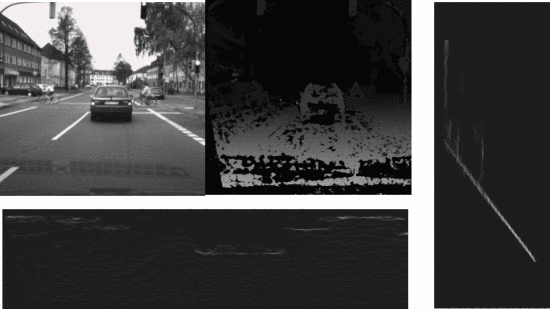
\includegraphics[width=0.80\textwidth, height=0.45\textwidth]{resources/png/uv_disparity.png}
    \caption{Recorded image, disparity image and UV-disparity maps.~\cite{withMain}~\label{figInit}}
\end{figure}

As shown in Figure, due to the constrains of the disparity maps, the horizontal one will have the same amount
of rows as the original image, and the number of columns will represent the total amount of possible disparity
values. The vertical map on the other hand is flipped, with the disparity values being encoded as each row of
the matrix.

\subsubsection{Adaptive thresholding}

This technique makes use of the stereo vision system characteristics, in order to classify obstacle pixels 
from the disparity map not through a fixed threshold, but through one tailored specifically for the detection
capabilities of the cameras. For this, the following characteristics are taken into account:
\begin{itemize}
    \item \(Y_{3dmin}\) - minimum height of the physical obstacle
    \item \(y_{min}\) - minimum projection height
    \item \(F\) - focal length of the cameras
    \item \(Z\) - obstacle depth
    \item \(B\) - baseline distance between the cameras
    \item \(d\) - disparity value of the pixel
\end{itemize}

In order to determine the threshold, the following equalities are taken into account~\cite{withMain}:
\begin{equation}
    \frac{y_{min}}{F} = \frac{Y_{3dmin}}{Z} 
\end{equation}
\begin{equation}
    y_{min} = \frac{F * Y_{3dmin}}{Z} 
\end{equation}
\begin{equation}
    Z = \frac{F * B}{d} 
\end{equation}

Resulting in the formula for determining \(y_{min}\) as:
\begin{equation}
    y_{min} = \frac{Y_{3dmin} * d}{B} 
\end{equation}

From this, the threshold value for distant pixels can be computed based on the values of \(y_{min}\) and 
\(Y_{3dmin}\), such that if the disparity value is small, it cannot be influenced by perceived noise.

\subsubsection{Vertical enhancement}

This step refers to the scan of each disparity column, both top-down and bottom-up, and identifying obstacle pixels.
If such a pixel is found, its pixel neighborhood is scanned, and similar disparities are considered as part of the
same obstacle.

\begin{figure}[H]
    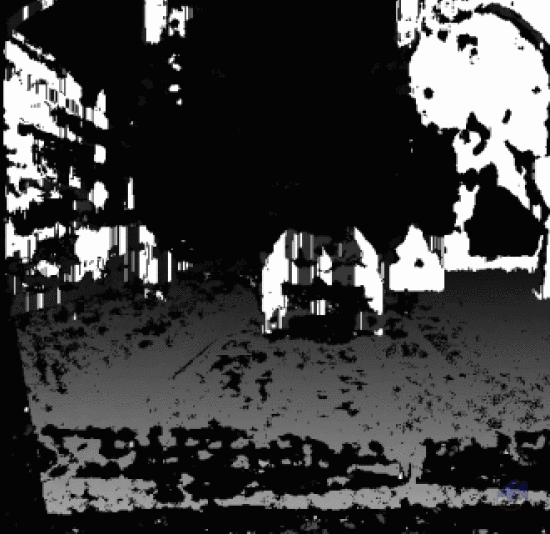
\includegraphics[width=0.50\textwidth, height=0.45\textwidth]{resources/png/vertical_enhancement.png}
    \caption{Vertical enhancement result.~\cite{withMain}~\label{figVert}}
\end{figure}

\subsubsection{Horizontal enhancement}

As the final step of the algorithm, it scans the v-disparity map in order to separate the road surface from any 
potential obstacles. As seen in {Figure uv disparity}, the road surface is most visible in the v-disparity map,
with the maximum value in each row being most likely a road pixel.

In order to extract the road profile from the v-disparity map, the following steps are taken:
\begin{itemize}
    \item Find the bottom-most row with a nonzero maximum.
    \item On the next row, add the row maximum to the road surface if its position is adjacent to the previous 
maximum.
    \item Stop the process if the profile becomes vertical, as it might overlap a vertical obstacle surface.
    \item If the current profile is beneath a threshold value, it is discarded and the process starts with the
next disparity map row that was not visited
\end{itemize}

\begin{figure}[H]
    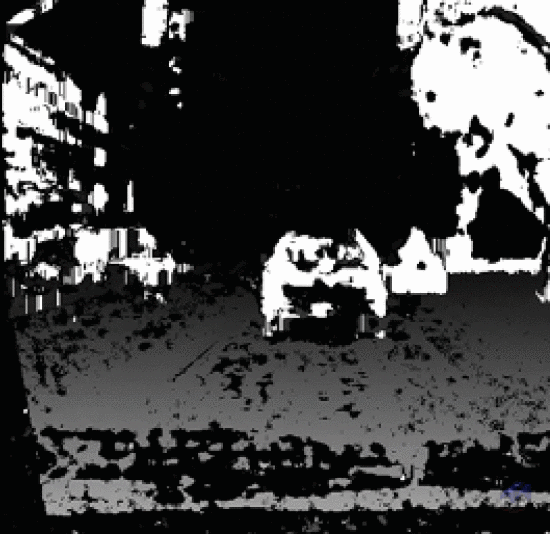
\includegraphics[width=0.50\textwidth, height=0.45\textwidth]{resources/png/horizontal_enhance.png}
    \caption{Horizontal enhancement result.~\cite{withMain}~\label{figHoriz}}
\end{figure}

\subsection{Results}

Implemented in C++, the algorithm was tested on an Intel I5 processor and resulted in a time of detection of 
\(4ms\), including the determination of the \(U\) and \(V\) disparity maps. As seen in the bellow images, 
each step of the algorithm improves upon the result of its antecedent, resulting in an efficient and reliable
detection of roadside obstacles for autonomous vehicles. 

\begin{figure}[H]
    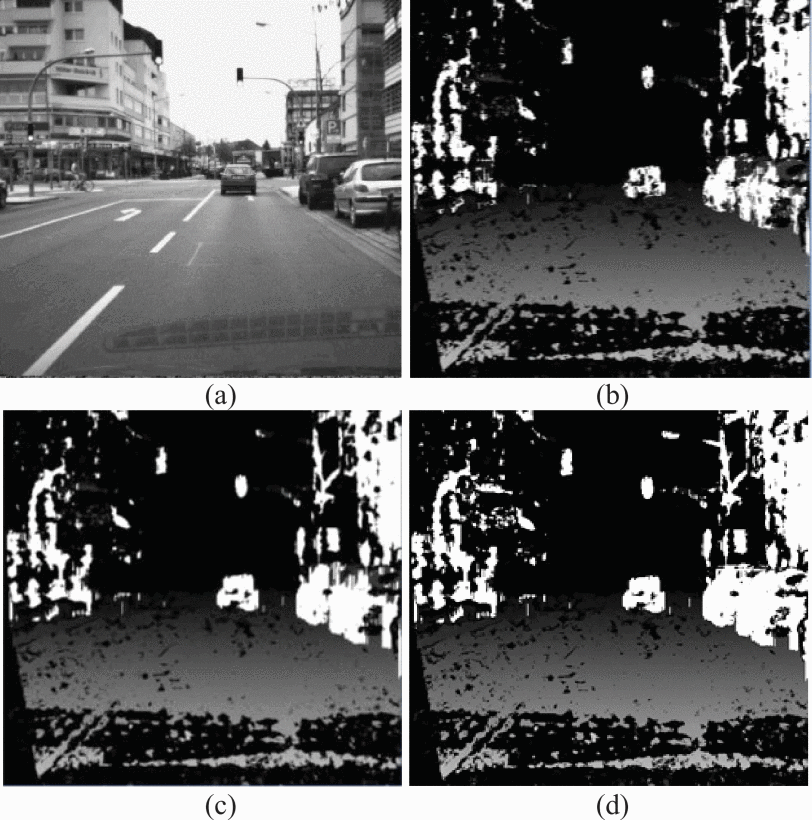
\includegraphics[width=0.50\textwidth, height=0.45\textwidth]{resources/png/final_result.png}
    \caption{Final result after all processing steps.~\cite{withMain}~\label{figSteps}}
\end{figure}